\documentclass[12pt]{article}
\usepackage{longtable}
\usepackage{makecell}
\usepackage{float}
\usepackage{graphicx}
\usepackage{bm}
\usepackage{placeins}
\usepackage{booktabs}
\usepackage{gensymb}
\usepackage{amssymb}
\usepackage{indentfirst}
\usepackage{threeparttable} 
\usepackage{multirow}
\usepackage{aligned-overset}
\usepackage[slantfont,boldfont]{xeCJK}
\usepackage{fontspec}
\renewcommand{\arraystretch}{1.5}
\usepackage[paperwidth=23cm,paperheight=37.21cm]{geometry}
\setCJKmainfont{SimSun}
\setmainfont{SimSun}
\setsansfont{SimSun}
% 设置正文字体为四号（12pt）
% \renewcommand{\CJKmainfont}{SimSun}
\renewcommand{\CJKfamilydefault}{\CJKrmdefault}
\renewcommand{\normalsize}{\fontsize{12pt}{18pt}\selectfont}
\normalsize

\title{用毛细管法测定液体的粘滞现象实验报告}
\author{2411545 邱凯锐}
\date{2025.10.10}

\begin{document}
\maketitle
\section{目的要求}
1. 了解粘滞现象的基本规律及粘滞系数的测定方法；

2. 根据泊肃叶公式测定水的粘滞系数；

3. 熟悉运用度数显微镜测微小长度。

\section{实验原理}
本实验是让水从毛细管中流过，通过测水的流量，根据泊肃叶公式求出表征水的粘度大小的粘滞系数。

粘滞系数为 $\eta$ 的液体，在内积均匀的毛细管中做层流运动时， $t$ 秒内流经毛细管任一截面的体积为：
\begin{equation}
    V=\frac{\pi D^4 \Delta p t}{128 l\eta}
\end{equation}

式（1）即泊肃叶公式。其中， $D$ 为毛细管直径， $l$ 为毛细管长度， $\Delta p$ 为毛细管两端的压力差。

证明如下：

\begin{figure}[H]
    \centering
    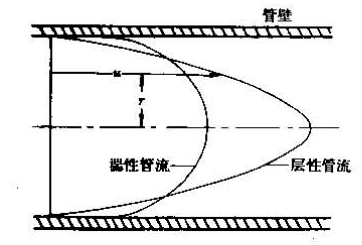
\includegraphics[width=0.65\textwidth]{1(1).png}
    \caption{流体速度分布}
\end{figure}

我们选取柱坐标系 $\{r,\phi,z\}$ ,管轴沿 $z$ 方向，半径 $R$ ，长度为 $l$ 。并假设流速 $u(r)$ 称轴对称分布，且满足以下边界条件

\begin{equation}
    \begin{cases}
        \left. u(r) \right|_{r=R}=0\\
        \left. \frac{\mathrm du(r)}{\mathrm dr}\right|_{r=0}=0
    \end{cases}
\end{equation}
粘滞力
\begin{equation}
    \mathrm d f=2\pi l\eta \mathrm d \left(r \frac{\mathrm du}{\mathrm dr} \right)
\end{equation}
压强差
\begin{equation}
    \mathrm d F= 2\pi (p_1-p_2) r\mathrm dr
\end{equation}
重力分量
\begin{equation}
    \mathrm dw \sin\alpha=\rho g\cdot 2\pi rl\mathrm dr \sin\alpha
\end{equation}

根据受力平衡可以得到
\begin{equation}
    -\mathrm df=\mathrm dF +\mathrm dw\sin\alpha
\end{equation}
代入式（3）、（4）、（5）得到
\begin{equation}
    -2\pi l\eta \mathrm d \left(r \frac{\mathrm du}{\mathrm dr} \right)=2\pi (p_1-p_2) r\mathrm dr+\rho g\cdot 2\pi rl\mathrm dr \sin\alpha
\end{equation}
对两边求积分得到
\begin{equation}
    -2\pi l\eta r\frac{\mathrm du}{\mathrm dr}=\pi \left(p_1-p_2+\rho gl \right) r^2
\end{equation}
化简之后再次积分
\begin{equation}
    u=\frac{(p_1-p_2+\rho gl)}{4l\eta}(R^2-r^2)
\end{equation}
令 $\Delta p=p_1-p_2+\rho gl$，计算流量 $Q$
% \begin{equation}
\begin{align}
    Q&=\int_S u\mathrm dS=\int_{0}^{R} \frac{\Delta p}{4l\eta} (R^2-r^2)\cdot 2\pi r\mathrm dr\\
     &=\frac{\pi \Delta pR^4}{8l\eta}
\end{align}
% \end{equation} 
在一定时间内流出的体积为
\begin{equation}
    V=Qt=\frac{\pi \Delta p D^4t}{128l\eta}
\end{equation}

若以 $h_1,h_2$ 分别表示容器内开始及停止计时的瞬间所对应的液面高度，而以 $h_0$ 表示毛细管的出口高度，则
\begin{equation}
    \Delta p=p_1-p_2+\rho gl=\rho g\left[\frac{1}{2}(h_1+h_2)-h_0\right]
\end{equation}

将式（12）改写为
\begin{equation}
    \eta=\frac{\pi D^4\Delta pt}{128lV}
\end{equation}

式（14）即为粘滞系数的计算式。式右侧诸量均可在实验中测得。其中， $\Delta p$ 按式（13）计算。

同时有经验公式
\begin{equation}
    \eta_\theta=a(b+\theta)^{-c}
\end{equation}
其中，$\eta_theta$ 为流体在 $\theta~^\circ\mathrm{C}$ 时的粘度，$a,b,c$ 为因液体种类或温度范围而异的常数。对水而言，当 $a=0.60070,b=43.252$ 及 $c=1.5423$ ，稳定在 $0~^\circ\mathrm{C}\sim 100~^\circ\mathrm{C}$ 范围内，与精确实验结果的误差不大于 $0.40\%$ 。因此，式（15）可以用来验证我们的实验结果。

\section{实验仪器}

（1）毛细管粘滞计

（2）读数显微镜

（3）$0~^\circ\mathrm C\sim 100~^\circ\mathrm C$ 温度计

（4）秒表

（5）烧杯

（6）待测液体：水

\begin{figure}[h]
    \centering
    
\includegraphics[width=0.5\textwidth]{3.jpg}
    \caption{毛细管粘滞计}
\end{figure}

\section{实验内容及实验数据}

1.用读数显微镜分别在不同位置的互垂方向测量毛细管两端样品的直径各四次，然后求其平均值 $D$ 。


\begin{table}[H]
    \centering
    \caption{内径 $D$ 数据}
    \vspace{2pt}
    \begin{minipage}{0.7\textwidth}
        \raggedleft
        放大率 $V=2$，$\Delta_D=0.001\ \mathrm{mm}$ 
    \end{minipage}\\[2pt]
    \begin{tabular}{cccc}
        $i$  & $a/\mathrm{mm}$     & $b/\mathrm{mm}$     & $D=\frac{|b-a|}{\sqrt 2V}/\mathrm{mm}$   \\ \hline \hline
        1 & 2.282 & 5.405 & 1.104147239 \\ \hline
        2 & 2.054 & 5.23  & 1.122885569 \\ \hline
        3 & 2.128 & 5.322 & 1.12924953  \\ \hline
        4 & 2.152 & 5.358 & 1.13349217  \\ \hline
        5 & 2.542 & 5.724 & 1.125006889 \\ \hline
        6 & 2.584 & 5.759 & 1.122532015 \\ \hline
        7 & 2.649 & 5.803 & 1.115107394 \\ \hline
        8 & 2.611 & 5.793 & 1.125006889
    \end{tabular}
\end{table}

计算得到 $\bar{D}=1.122178462\ \mathrm{mm}$。计算 $A$ 类不确定度
\begin{equation}
    u_A=\sqrt{\frac{\sum_{i=1}^n(D_i-\bar D)^2}{n(n-1)}}=0.00392\ \mathrm{mm}
\end{equation}
$B$ 类不确定度
\begin{equation}
    u_B=\frac{\Delta_D}{\sqrt 3}=0.000557\ \mathrm{mm}
\end{equation}
合成不确定度
\begin{equation}
    u_D=\sqrt{u_A^2+u_B^2}=0.0040\ \mathrm{mm}
\end{equation}
得到 $D=1.1222\pm 0.0040\ \mathrm{mm} $

2. 调好仪器后，将预先准备好并已测得初温 $\theta_1$（接近室温 $\theta_e$）的待测样品由量水缓缓注入容器 $V$ 内，记录确认的液体体积 $V$（约 $50\,\mathrm{ml}$）流经毛细管所用的时间 $t$，并记下相应上、下液面及毛细管出口相对于参考面“0”的高度：$h_1, h_2$ 及 $h_0$。最后在接水容器（烧杯）内测出液体之末温 $\theta_2$。以相同体积 $V$ 及相同高度 $h_1, h_2$，重复测温度及流量三次，以期分别求出不同温度下该液体的粘滞系数。

实验数据：
$$
环境温度：\theta_e=\frac{\theta_{e1}+\theta_{e2}}{2}=19.9\ ~^\circ\mathrm C,\quad 水的密度：\rho=1000\ \mathrm{kg}\cdot\mathrm{m^{-3}}
$$
$$
重力加速度： g=9.8\ \mathrm{m\cdot s^{-2}},\quad 毛细管长度： l=0.30\ \mathrm m
$$
\begin{table}[h]
    \centering
    \renewcommand{\arraystretch}{1.3}
    \caption{粘滞系数测量数据}
    \begin{tabular}{c|c|c|c|c|c|c|c|c|c|c}
    \multirow{2}{*}{$i$} 
    & \multicolumn{3}{c|}{\textbf{水温} $\theta_i\, (^\circ\mathrm{C})$} 
    & \multirow{2}{*}{$h_1/ \mathrm{mm}$} 
    & \multirow{2}{*}{$h_2/ \mathrm{mm}$} 
    & \multirow{2}{*}{$h_0/ \mathrm{mm}$} 
    & \multirow{2}{*}{$\Delta p/ \mathrm{Pa}$} 
    & \multirow{2}{*}{$V/ \mathrm{mL}$} 
    & \multirow{2}{*}{$t_i/ \mathrm{t}$} 
    & \multirow{2}{*}{$\eta_i/ \mathrm{mPa\cdot s}$} \\ \cline{2-4}
    & $\theta_{i1}$ & $\theta_{i2}$ & $\bar{\theta}_i$ &  &  &  &  &  &  &  \\ \hline \hline
    1 & 19.7 & 19.9 & 19.8 & 29.00 & 21.50 & 2.00 & 2278.5 & 50 & 180.33 & 1.066138 \\ \hline 
2 & 20.3 & 19.9 & 20.1 & 29.00 & 21.50 & 2.00 & 2278.5 & 50 & 181.75 & 1.074533 \\ \hline
3 & 19.9 & 19.9 & 19.9 & 29.00 & 21.50 & 2.00 & 2278.5 & 50 & 180.18 & 1.065251 
    \end{tabular}
\end{table}

选取第一次实验计算不确定度。$h_1,h_2,h_0$ 有 $B$ 类不确定度，
\begin{equation}
    u_{hB}=u_{h_1}=u_{h_2}=u_{h_0}=\frac{\Delta_h}{\sqrt 3}= 0.5773\ \mathrm{mm}
\end{equation}
得到 $\Delta p$ 的不确定度为
\begin{equation}
    u_{\Delta p}=\rho g \frac{u_{hB}}{\sqrt{2}}=4.0005\ \mathrm{Pa}
\end{equation}
体积 $V$ 的不确定度为
\begin{equation}
    u_V=\frac{\Delta_V}{\sqrt 3}=0.5773\ \mathrm{mL}
\end{equation}
时间 $t$ 的不确定度包括电子秒表的不确定度和人的反应时间
\begin{equation}
    u_t=\sqrt{\left(\frac{\Delta_t}{\sqrt 3}\right)^2+\left(\frac{0.2}{\sqrt 3}\right)^2}=0.1154\ \mathrm{s}
\end{equation}
最后合成得到 $\eta$ 的不确定度为
\begin{equation}
    u_{\eta}=\eta\sqrt{\left(4\frac{u_D}{D} \right)^2+\left(\frac{u_{\Delta p}}{\Delta p} \right)^2+\left(\frac{u_t}{t} \right)^2+\left(\frac{u_V}{V} \right)^2}=0.020\ \mathrm{mPa\cdot s}
\end{equation}

根据经验公式（15）计算得到
\begin{equation}
    \eta_{\theta}=1.00689\ \mathrm{mPa\cdot s}
\end{equation}
相对误差为
\begin{equation}
    E=\frac{|\eta-\eta_{\theta}|}{\eta_{\theta}}\times 100\%=5.88\%
\end{equation}
不确定度产生的主要原因有：

（1）毛细管孔不是完美的圆形，且读数显微镜测量稳定性较差，测量内径 $D$ 时存在较大误差；

（2）在读取液体体积 $V$ 时，时间较为紧迫，导致产生的误差也较大；

（3）液面的高度差使用刻度尺较难测量，测量过程较为粗糙。

\section{思考题}

（1） 粘滞系数 $\eta$ 与开始计时的液面高度有关吗？

我们将式（13）改写为与 $t$ 有关的函数
\begin{equation}
    \Delta p(t)=\rho g(h(t)-h_0)
\end{equation}
假设液面的截面积为 $S$ ，那么有
\begin{equation}
    -\mathrm dh=\frac{Q(t)\mathrm dt}{S}=\frac{\pi D^4\Delta p(t)}{128l\eta S} \mathrm dt=\frac{\pi D^4 \rho g}{128l\eta}(h-h_0)\mathrm dt
\end{equation}
积分得到
\begin{equation}
    \ln(\frac{h_1-h_0}{h-h_0})=\frac{\pi D^4 \rho gt}{128l\eta S}
\end{equation}
令 $\alpha=\frac{\pi D^4 \rho g}{128l\eta S}$,解得
\begin{equation}
    h(t)=e^{-\alpha t}(h_1-h_0)+h_0
\end{equation}
重新计算流出液体的体积 
\begin{equation}
    V'=S[h_1-h(t)]=(1-e^{-\alpha t})(h_1-h_0)S
\end{equation}
以及重写式（12）
\begin{equation}
    V=S\alpha \left( \frac{h_1+h(t)}{2}-h_0\right)=\alpha\left(e^{-\alpha t}-\frac12\right)(h_1-h_0)S
\end{equation}

可以看出在毛细管法下,开始计时的液面高度会影响粘滞系数 $\eta$ 测量的大小。但如果测量 $h(t)-h_0$ 的时间常数 $\tau$ 满足 $\alpha\tau= 1$,即可得到
\begin{equation}
    \eta = \frac{\pi D^4\rho g}{128 lS\alpha}=\frac{\pi D^4\rho g\tau}{128lS}
\end{equation} 
与 $h_1$ 无关。

（2） 计算本次实验条件下的雷诺数，以验证是否满足泊肃叶公式成立的条件。

雷诺数
\begin{equation}
    R_e=\frac{\rho \bar u D}{\eta}=295< 2000
\end{equation}
满足泊肃叶公式的成立条件。

\begin{figure}[H]
    \centering
    
\includegraphics[width=0.6\textwidth]{2.jpg}
    \caption{原始数据}
\end{figure}

\end{document}

